Biomechanics researchers rely on numerical simulations of motion to gain understanding on a variety of scientific topics such as the physiological causes of movement disorders and their consequences on health \cite{pizzolato2015ceinms}, the estimation of non-measurable physiological quantities (e.g., muscle forces \cite{bailly2020real}) and the optimality of human movement \cite{porsa2016direct}.
The musculoskeletal models used in these simulations generally have a large number of degrees of freedom and they are governed by several ordinary differential equations (ODEs) which mainly describe multibody and muscle activation dynamics.
The complexity of these systems has led scientists to formulate their simulations as optimal control problems (OCP), relying on efficient non-linear optimization software to find trajectories that fulfill a desired task while enforcing the system dynamics and minimizing a cost (e.g. motion duration, energy expenditure, matching experimental data, etc.).
Up to very recently, there was no off-the-shelf software available to the community to quickly formulate and solve such musculoskeletal OCPs \cite{Charles2013}. 
Consequently, researchers had to develop their own solutions, with little or no dissemination to the community, limiting  synergies between researchers.
\begin{figure}[t!]
\centering
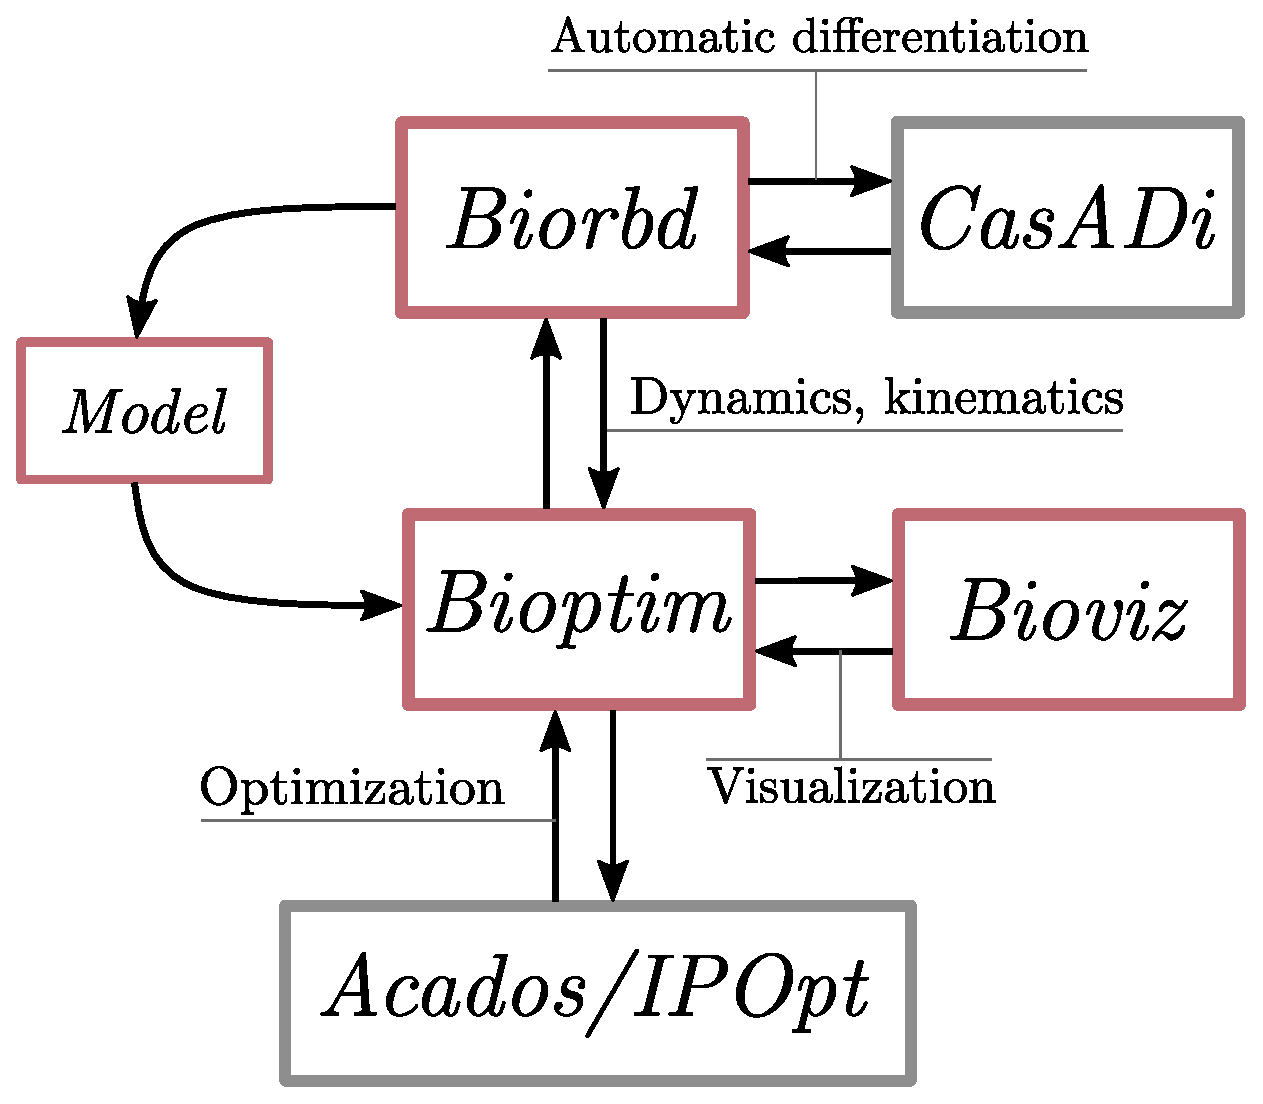
\includegraphics[width=0.9\columnwidth]{figures/dependencies.eps}
\caption{\bioptim dependencies flowchart. The red-boxed software are developed by the S2M team. The \bioptim part is further detailed in Fig.~\ref{fig:flowchart}.}
\label{fig:dependencies}
\vspace*{-0.8cm}
\end{figure}

As a result, many approaches coexist to formulate and solve OCPs in the biomechanical literature. 
The formulation, also called discretization, consists in turning a continuous trajectory optimization problem into a generic discrete non-linear program (NLP) that is solved using a dedicated algorithm. 
The main family of so-called \textit{direct} transcription methods comes from numerical optimal control. 
They consist in straightforwardly choosing the state and/or the control as optimization variables at a given number of points along the trajectory and they rely on the integration of the system dynamics between these points. 

For instance, the \textit{direct collocation} method has shown its efficiency in some studies investigating human motion \cite{febrer-nafriaComparisonDifferentOptimal2020, ezatiComparisonDirectCollocation2020}.
It consists in approximating the integration of the system dynamics using polynomials that describe the state and control trajectories.
Its main advantages are that it leads to very sparse NLPs, that knowledge about the state trajectory can be used in the initialization, and that it handles unstable systems well. 
Its major disadvantage is that adaptive integration error control implies regridding the whole problem and thus changes the NLP dimensions~\cite{diehl2006fast}.
\textit{Direct multiple shooting} is another direct method that was also applied with success in a lot of biomechanics \cite{koschorreck2012modeling, felis2013modeling, charbonneau2020optimal, bailly2020optimal} and robotics \cite{diehl2006fast, giftthaler2018control, bailly2018mechanical} studies.
Its advantages are mostly the same as for direct collocation in addition to combining integration error control with fixed NLP dimensions, as it relies on possibly adaptive ODE solvers to integrate the system dynamics.
Besides direct methods, other choices can be made, as in \cite{yeadon2000mechanics, begon2009effect}, where the optimization variables are instants at which a switch in the motor strategy occurs, using polynomials function (4th, 5th order) in-between, or in \cite{leboeuf2006energetic, huchez2015local}, where the optimization variables are the coefficients of fourth order polynomial approximations of the states, with linking conditions to enforce the continuity of the controls. 
These last approaches are less generic than the direct methods as they either require a prior knowledge about the state and control trajectories. 
Most of the time, when investigating complex biomechanics issues, we do not have this information. 

Concerning the non-linear solver, a variety of software exist and have been used to solve transcribed musculoskeletal NLPs.
They can use different heuristics: interior point methods (\ipopt, \cite{wachter2006implementation}) or sequential quadratic programming (\textit{snopt} \cite{gill2005snopt}, \acados \cite{verschueren2018towards}), but they are all gradient based.
Therefore, derivatives of the NLP cost function and constraints are required to perform optimization.
These derivatives can be obtained by finite differences (often implemented but inaccurate thus comprising convergence) or computed exactly using automatic differentiation (requiring to write all dependencies of the software in symbolic variables), using, e.g., \casadi \cite{andersson2019casadi}.

In order to promote the use of musculoskeletal optimal control among biomechanics researcher, we identified a strong need for a dedicated tool, as shown by the recently launched \moco \cite{dembia2020opensim}. 
The biomechanics community being mainly composed of software users, such a tool should request a flexible user interface written in a widely used high-level and if possible open-source language (e.g. Python) with a low-level core (e.g. C++) for efficiency. 

To develop such a software, four interrelated components are essential in our opinion: \textit{i)} a musculoskeletal modeling software, with a visualization module (multibody kinematics and dynamics, muscle dynamics, etc.), \textit{ii)} a method for automatic differentiation, \textit{iii)} a discretization approach, and \textit{iv)} one or several nonlinear programming (NLP) solvers. 
General-purpose optimal control software (e.g. \gpopsii \cite{patterson2014gpops}, \muscodii \cite{leineweber2003efficient1,leineweber2003efficient2}, \acado \cite{houska2011acado}]) address \textit{ii)} to \textit{iv)} but they need to be interfaced with a musculoskeletal modeling module and they do not provide any built-in biomechanics features (physiological cost functions, kinematic constraints, etc.). 
In that sense, the aforementioned \moco, is a welcome initiative that draws its strength from its integration with the widely used \opensim.
However, it faces the following limitations: it uses finite differences to avoid the complexity of adapting the \opensim codebase to support automatic differentiation, it uses direct collocation as transcription method, preventing the use of adaptive ODE solvers and it is not as flexible as required by the community, since it requires the user to develop new features, such as new objective functions, in C++.\\
\newpage

The objective of the present paper is to introduce \bioptim\footnote{
\href{https://github.com/pyomeca/bioptim}{https://github.com/pyomeca/bioptim}}, an open-source optimal control software dedicated to musculoskeletal biomechanics.
\bioptim is based on C++ code for computational efficiency but the user interface is written in Python for flexibility and ease-of-use. 
The OCP transcription uses direct multiple shooting to preserve the possibility of using arbitrarily accurate ODE solvers for the integration, which is fully parallelized for more efficiency.
\bioptim's core is fully written in \casadi symbolics to benefit from algorithmic differentiation and to exploit \casadi 's interface with several non-linear solvers (\ipopt, \snopt).
Moreover, \bioptim is interfaced with the cutting-edge solver \acados, a recent NLP solver dedicated to direct multiple shooting, intended for real-time applications.
The purpose of \bioptim is to allow fast and flexible musculoskeletal OCP formulation and solving by providing a framework with a lot of typical biomechanics problem already implemented and customizable.

The paper is organized as follows: first, the design and implementation of \bioptim are described.
Next, the versatility and performances of \bioptim are shown through a variety of examples available online. 
